\documentclass{memoir}

\usepackage[top=1in,bottom=1in,left=1in,right=1in,letterpaper]{geometry}
\usepackage{graphicx}

\begin{document}
\frontmatter
\includegraphics[width=\textwidth]{cover.png}
\thispagestyle{empty}
\newpage

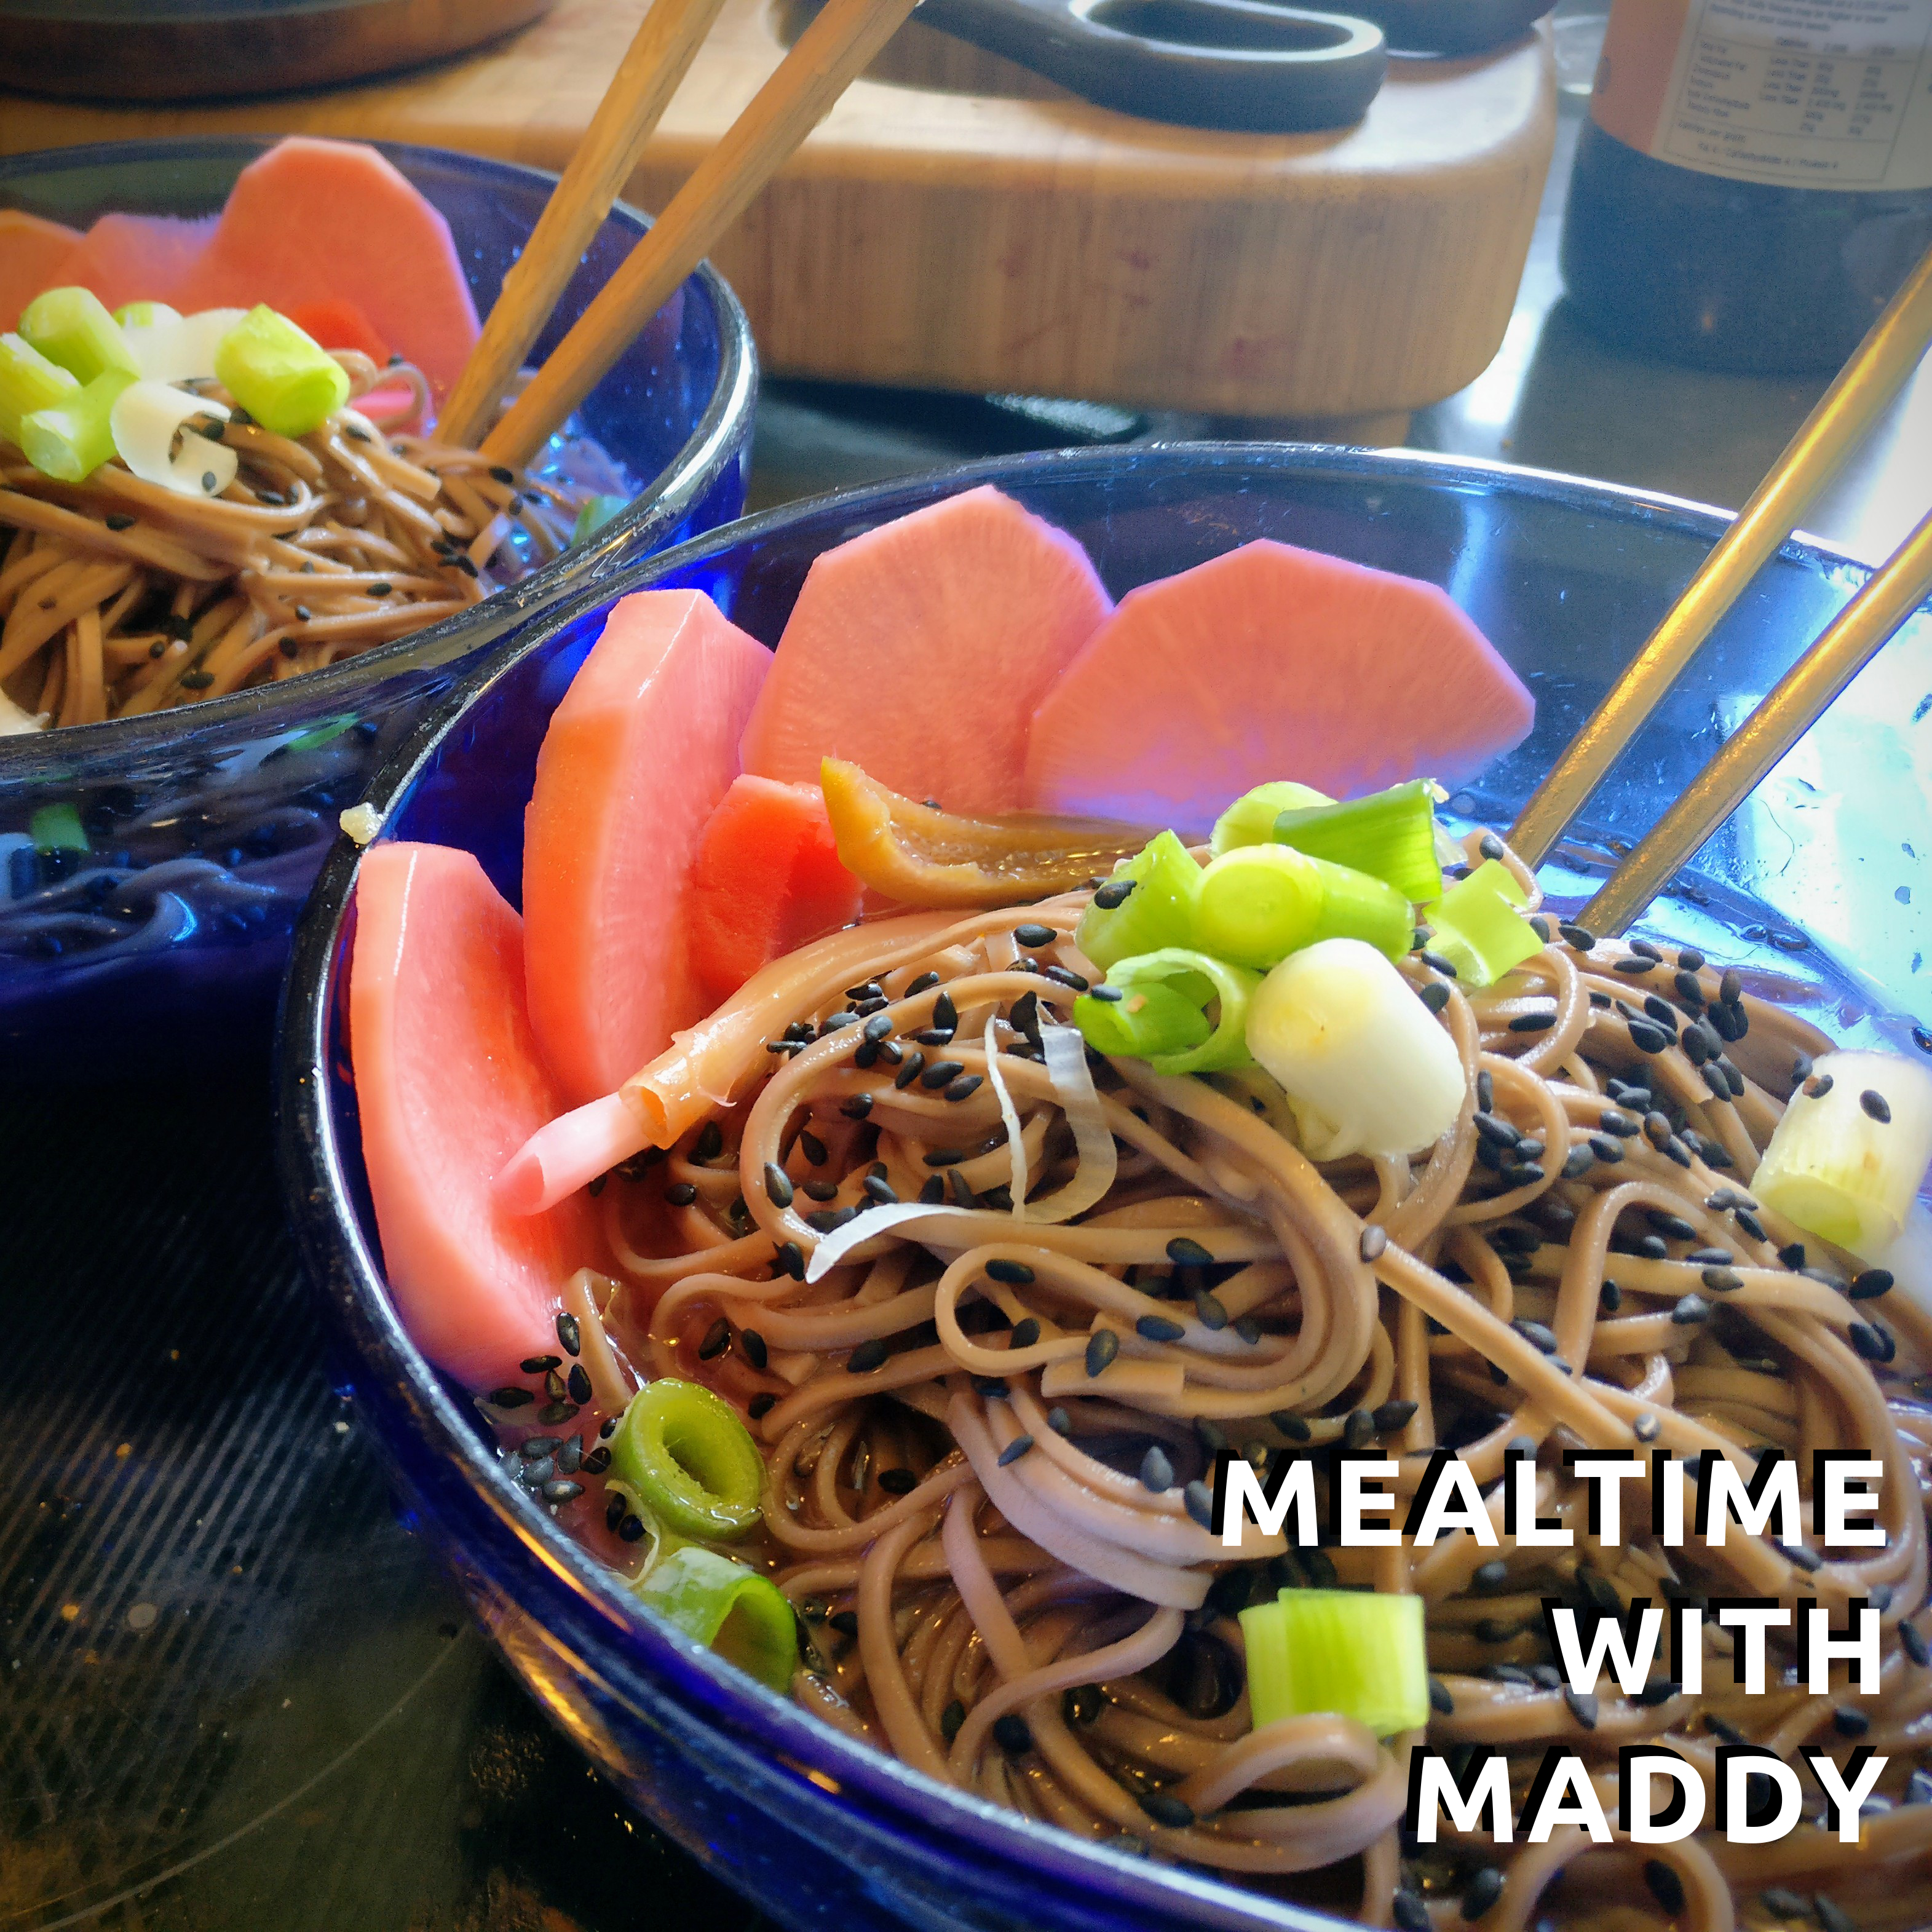
\includegraphics[width=\textwidth]{inner-cover.png}
\thispagestyle{empty}
\newpage

% Title page

\tableofcontents*

\chapter*{Dedication}

\begin{verse}
  To the polycule\\
  \vin JD and Robin and Lexy\\
  To Jenn\\
  To the dogs\\
  \vin Zephyr and Falcon\\
  and to the idea\\
  \vin if not exactly the implementation\\
  \vin \vin of Twitter.
\end{verse}

\chapter{About}

\mainmatter

\chapter*{Bananas Foster}
\renewcommand{\chaptertitle}{Bananas Foster}
\addcontentsline{toc}{chapter}{\hspace{1.5ex}Bananas Foster}

\includegraphics[height=\textwidth-1.3in]{food/bananas-foster/images/hi-res/01.jpg}
\newpage
\includegraphics[width=\textwidth]{food/bananas-foster/images/hi-res/02.jpg}
\newpage
\includegraphics[width=\textwidth]{food/bananas-foster/images/hi-res/03.jpg}
\newpage
\includegraphics[width=\textwidth]{food/bananas-foster/images/hi-res/04.jpg}
\newpage
\includegraphics[width=\textwidth]{food/bananas-foster/images/hi-res/05.jpg}
\newpage
\includegraphics[width=\textwidth]{food/bananas-foster/images/hi-res/06.jpg}
\newpage
\includegraphics[height=\textheight]{food/bananas-foster/images/hi-res/07.jpg}
\newpage
\includegraphics[width=\textwidth]{food/bananas-foster/images/hi-res/08.jpg}
\newpage
\includegraphics[width=\textwidth]{food/bananas-foster/images/hi-res/09.jpg}
\newpage
\includegraphics[width=\textwidth]{food/bananas-foster/images/hi-res/10.jpg}


\chapter*{Bananas Foster}
\renewcommand{\chaptertitle}{Bananas Foster}
\addcontentsline{toc}{chapter}{\hspace{1.5ex}Bananas Foster}

\includegraphics[height=\textwidth-1.3in]{food/bananas-foster/images/hi-res/01.jpg}
\newpage
\includegraphics[width=\textwidth]{food/bananas-foster/images/hi-res/02.jpg}
\newpage
\includegraphics[width=\textwidth]{food/bananas-foster/images/hi-res/03.jpg}
\newpage
\includegraphics[width=\textwidth]{food/bananas-foster/images/hi-res/04.jpg}
\newpage
\includegraphics[width=\textwidth]{food/bananas-foster/images/hi-res/05.jpg}
\newpage
\includegraphics[width=\textwidth]{food/bananas-foster/images/hi-res/06.jpg}
\newpage
\includegraphics[height=\textheight]{food/bananas-foster/images/hi-res/07.jpg}
\newpage
\includegraphics[width=\textwidth]{food/bananas-foster/images/hi-res/08.jpg}
\newpage
\includegraphics[width=\textwidth]{food/bananas-foster/images/hi-res/09.jpg}
\newpage
\includegraphics[width=\textwidth]{food/bananas-foster/images/hi-res/10.jpg}


\chapter{Preserved Lemons --- Part 1}


\chapter*{Bananas Foster}
\renewcommand{\chaptertitle}{Bananas Foster}
\addcontentsline{toc}{chapter}{\hspace{1.5ex}Bananas Foster}

\includegraphics[height=\textwidth-1.3in]{food/bananas-foster/images/hi-res/01.jpg}
\newpage
\includegraphics[width=\textwidth]{food/bananas-foster/images/hi-res/02.jpg}
\newpage
\includegraphics[width=\textwidth]{food/bananas-foster/images/hi-res/03.jpg}
\newpage
\includegraphics[width=\textwidth]{food/bananas-foster/images/hi-res/04.jpg}
\newpage
\includegraphics[width=\textwidth]{food/bananas-foster/images/hi-res/05.jpg}
\newpage
\includegraphics[width=\textwidth]{food/bananas-foster/images/hi-res/06.jpg}
\newpage
\includegraphics[height=\textheight]{food/bananas-foster/images/hi-res/07.jpg}
\newpage
\includegraphics[width=\textwidth]{food/bananas-foster/images/hi-res/08.jpg}
\newpage
\includegraphics[width=\textwidth]{food/bananas-foster/images/hi-res/09.jpg}
\newpage
\includegraphics[width=\textwidth]{food/bananas-foster/images/hi-res/10.jpg}


\chapter*{Bananas Foster}
\renewcommand{\chaptertitle}{Bananas Foster}
\addcontentsline{toc}{chapter}{\hspace{1.5ex}Bananas Foster}

\includegraphics[height=\textwidth-1.3in]{food/bananas-foster/images/hi-res/01.jpg}
\newpage
\includegraphics[width=\textwidth]{food/bananas-foster/images/hi-res/02.jpg}
\newpage
\includegraphics[width=\textwidth]{food/bananas-foster/images/hi-res/03.jpg}
\newpage
\includegraphics[width=\textwidth]{food/bananas-foster/images/hi-res/04.jpg}
\newpage
\includegraphics[width=\textwidth]{food/bananas-foster/images/hi-res/05.jpg}
\newpage
\includegraphics[width=\textwidth]{food/bananas-foster/images/hi-res/06.jpg}
\newpage
\includegraphics[height=\textheight]{food/bananas-foster/images/hi-res/07.jpg}
\newpage
\includegraphics[width=\textwidth]{food/bananas-foster/images/hi-res/08.jpg}
\newpage
\includegraphics[width=\textwidth]{food/bananas-foster/images/hi-res/09.jpg}
\newpage
\includegraphics[width=\textwidth]{food/bananas-foster/images/hi-res/10.jpg}


\chapter{Preserved Lemons --- Part 2}


\chapter*{Shakshouka}
\renewcommand{\chaptertitle}{Shakshouka}
\addcontentsline{toc}{chapter}{\hspace{1.5ex}Shakshouka}


\chapter*{Tamago Kake Gohan}
\renewcommand{\chaptertitle}{Tamago Kake Gohan}
\addcontentsline{toc}{chapter}{\hspace{1.5ex}Tamago Kake Gohan}

TIP reheating rice


\chapter*{Kimchi: Part 1}
\renewcommand{\chaptertitle}{Kimchi: Part 1}
\addcontentsline{toc}{chapter}{\hspace{1.5ex}Kimchi: Part 1}

Getting baek kimchi to spice/age, getting mulkimchi to salt and wait


\chapter*{Bananas Foster}
\renewcommand{\chaptertitle}{Bananas Foster}
\addcontentsline{toc}{chapter}{\hspace{1.5ex}Bananas Foster}

\includegraphics[height=\textwidth-1.3in]{food/bananas-foster/images/hi-res/01.jpg}
\newpage
\includegraphics[width=\textwidth]{food/bananas-foster/images/hi-res/02.jpg}
\newpage
\includegraphics[width=\textwidth]{food/bananas-foster/images/hi-res/03.jpg}
\newpage
\includegraphics[width=\textwidth]{food/bananas-foster/images/hi-res/04.jpg}
\newpage
\includegraphics[width=\textwidth]{food/bananas-foster/images/hi-res/05.jpg}
\newpage
\includegraphics[width=\textwidth]{food/bananas-foster/images/hi-res/06.jpg}
\newpage
\includegraphics[height=\textheight]{food/bananas-foster/images/hi-res/07.jpg}
\newpage
\includegraphics[width=\textwidth]{food/bananas-foster/images/hi-res/08.jpg}
\newpage
\includegraphics[width=\textwidth]{food/bananas-foster/images/hi-res/09.jpg}
\newpage
\includegraphics[width=\textwidth]{food/bananas-foster/images/hi-res/10.jpg}


\chapter{Kimchi --- Part 2}

Finishing mulkimchi prep with broth, flip baek kimchi


\chapter{Sichuan Dry-Fried String Beans}

TIP make extra oil


TIP make extra oil

\chapter*{Kimchi: Part 3}
\renewcommand{\chaptertitle}{Kimchi: Part 3}
\addcontentsline{toc}{chapter}{\hspace{1.5ex}Kimchi: Part 3}

jarring baek kimchi


Jarring baek kimchi

\chapter{Mul-naengmyeon}

Using mulkimchi


Using mulkimchi

\chapter*{Okonomiyaki}
\renewcommand{\chaptertitle}{Okonomiyaki}
\addcontentsline{toc}{chapter}{\hspace{1.5ex}Okonomiyaki}

TIP using kimchi for kimchijeon


TIP use baek kimchi

\chapter*{Bananas Foster}
\renewcommand{\chaptertitle}{Bananas Foster}
\addcontentsline{toc}{chapter}{\hspace{1.5ex}Bananas Foster}

\includegraphics[height=\textwidth-1.3in]{food/bananas-foster/images/hi-res/01.jpg}
\newpage
\includegraphics[width=\textwidth]{food/bananas-foster/images/hi-res/02.jpg}
\newpage
\includegraphics[width=\textwidth]{food/bananas-foster/images/hi-res/03.jpg}
\newpage
\includegraphics[width=\textwidth]{food/bananas-foster/images/hi-res/04.jpg}
\newpage
\includegraphics[width=\textwidth]{food/bananas-foster/images/hi-res/05.jpg}
\newpage
\includegraphics[width=\textwidth]{food/bananas-foster/images/hi-res/06.jpg}
\newpage
\includegraphics[height=\textheight]{food/bananas-foster/images/hi-res/07.jpg}
\newpage
\includegraphics[width=\textwidth]{food/bananas-foster/images/hi-res/08.jpg}
\newpage
\includegraphics[width=\textwidth]{food/bananas-foster/images/hi-res/09.jpg}
\newpage
\includegraphics[width=\textwidth]{food/bananas-foster/images/hi-res/10.jpg}


\chapter*{Green Chili}
\renewcommand{\chaptertitle}{Green Chili}
\addcontentsline{toc}{chapter}{\hspace{1.5ex}Green Chili}

TIP snazzy beans


\chapter*{Bananas Foster}
\renewcommand{\chaptertitle}{Bananas Foster}
\addcontentsline{toc}{chapter}{\hspace{1.5ex}Bananas Foster}

\includegraphics[height=\textwidth-1.3in]{food/bananas-foster/images/hi-res/01.jpg}
\newpage
\includegraphics[width=\textwidth]{food/bananas-foster/images/hi-res/02.jpg}
\newpage
\includegraphics[width=\textwidth]{food/bananas-foster/images/hi-res/03.jpg}
\newpage
\includegraphics[width=\textwidth]{food/bananas-foster/images/hi-res/04.jpg}
\newpage
\includegraphics[width=\textwidth]{food/bananas-foster/images/hi-res/05.jpg}
\newpage
\includegraphics[width=\textwidth]{food/bananas-foster/images/hi-res/06.jpg}
\newpage
\includegraphics[height=\textheight]{food/bananas-foster/images/hi-res/07.jpg}
\newpage
\includegraphics[width=\textwidth]{food/bananas-foster/images/hi-res/08.jpg}
\newpage
\includegraphics[width=\textwidth]{food/bananas-foster/images/hi-res/09.jpg}
\newpage
\includegraphics[width=\textwidth]{food/bananas-foster/images/hi-res/10.jpg}


\chapter{Preserved Lemons --- Part 3}


\chapter*{Bananas Foster}
\renewcommand{\chaptertitle}{Bananas Foster}
\addcontentsline{toc}{chapter}{\hspace{1.5ex}Bananas Foster}

\includegraphics[height=\textwidth-1.3in]{food/bananas-foster/images/hi-res/01.jpg}
\newpage
\includegraphics[width=\textwidth]{food/bananas-foster/images/hi-res/02.jpg}
\newpage
\includegraphics[width=\textwidth]{food/bananas-foster/images/hi-res/03.jpg}
\newpage
\includegraphics[width=\textwidth]{food/bananas-foster/images/hi-res/04.jpg}
\newpage
\includegraphics[width=\textwidth]{food/bananas-foster/images/hi-res/05.jpg}
\newpage
\includegraphics[width=\textwidth]{food/bananas-foster/images/hi-res/06.jpg}
\newpage
\includegraphics[height=\textheight]{food/bananas-foster/images/hi-res/07.jpg}
\newpage
\includegraphics[width=\textwidth]{food/bananas-foster/images/hi-res/08.jpg}
\newpage
\includegraphics[width=\textwidth]{food/bananas-foster/images/hi-res/09.jpg}
\newpage
\includegraphics[width=\textwidth]{food/bananas-foster/images/hi-res/10.jpg}


\chapter*{Bananas Foster}
\renewcommand{\chaptertitle}{Bananas Foster}
\addcontentsline{toc}{chapter}{\hspace{1.5ex}Bananas Foster}

\includegraphics[height=\textwidth-1.3in]{food/bananas-foster/images/hi-res/01.jpg}
\newpage
\includegraphics[width=\textwidth]{food/bananas-foster/images/hi-res/02.jpg}
\newpage
\includegraphics[width=\textwidth]{food/bananas-foster/images/hi-res/03.jpg}
\newpage
\includegraphics[width=\textwidth]{food/bananas-foster/images/hi-res/04.jpg}
\newpage
\includegraphics[width=\textwidth]{food/bananas-foster/images/hi-res/05.jpg}
\newpage
\includegraphics[width=\textwidth]{food/bananas-foster/images/hi-res/06.jpg}
\newpage
\includegraphics[height=\textheight]{food/bananas-foster/images/hi-res/07.jpg}
\newpage
\includegraphics[width=\textwidth]{food/bananas-foster/images/hi-res/08.jpg}
\newpage
\includegraphics[width=\textwidth]{food/bananas-foster/images/hi-res/09.jpg}
\newpage
\includegraphics[width=\textwidth]{food/bananas-foster/images/hi-res/10.jpg}


\end{document}
